\subsubsection{Proxy}
\label{ssub:proxy}

Il pattern Proxy fornisce un surrogato di un altro oggetto per controllarne
l'accesso. Esso è applicabile ogni qualvolta vi sia bisogno di un più versatile
e sofisticato riferimento ad un oggetto rispetto a un semplice puntatore.

Un proxy è applicabile nelle seguenti situazioni:

\begin{itemize}
    \item Remote proxy: fornisce un rappresentante in locale di un oggetto in un
    diverso spazio di indirizzamento;
    \item Virtual proxy: crea oggetti complessi e pesanti on-demand;
    \item Protection proxy: controlla l'accesso all'oggetto originale;
    \item Smart reference: rimpiazza il semplice puntatore per svolgere azioni
    più avanzate, come il reference counting;
\end{itemize}

\begin{figure}[h!]
  \centering
  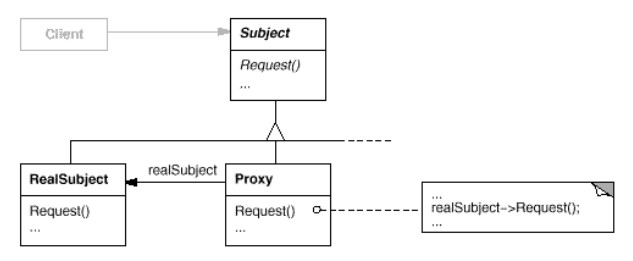
\includegraphics[scale=0.55]{imgs/proxy.jpg}
  \caption{Diagramma delle classi del pattern Proxy}
\end{figure}
